\documentclass{article}
\usepackage{tikz}
\usetikzlibrary{decorations.markings}

\begin{document}

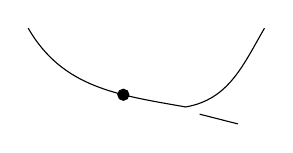
\begin{tikzpicture}[
    tangent/.style={
        decoration={
            markings,% switch on markings
            mark=
                at position #1
                with
                {
                    \coordinate (tangent point-\pgfkeysvalueof{/pgf/decoration/mark info/sequence number}) at (0pt,0pt);
                    \coordinate (tangent unit vector-\pgfkeysvalueof{/pgf/decoration/mark info/sequence number}) at (1,0pt);
                    \coordinate (tangent orthogonal unit vector-\pgfkeysvalueof{/pgf/decoration/mark info/sequence number}) at (0pt,1);
                }
        },
        postaction=decorate
    },
    use tangent/.style={
        shift=(tangent point-#1),
        x=(tangent unit vector-#1),
        y=(tangent orthogonal unit vector-#1)
    },
    use tangent/.default=1
]
%\draw [
%    tangent=0.4,
%    tangent=0.56
%] (0,0)
%    to [out=20,in=120] (5,2)
%    to [out=-60, in=110] (9,1);
%\draw [blue, thick, use tangent] (-3,0) -- (3,0);
%\draw [orange, thick, use tangent=2] (-2,0) -- (2,0) (0,0) -- (0,1);
%%%%%%%%%%%%%%%%%%%%%%%%%%%%%%%%%%%%%%%%%%%%%%%%%%%%%%%%%%%%%%%%%
%\draw[tangent=0.4] (1,1) to[out=70, in=200] (4,4);
%\filldraw[use tangent] (0,0) circle (2pt);
%\draw[use tangent] (-3,0) -- (2.5,0);
\draw[tangent=0.4] (.5,2)
to[out=-60,in=170] (2.5,1)
to[out=10,in=-120] (3.5,2);
\filldraw[use tangent] (0,0) circle (2pt);
\draw[use tangent] (1,0) -- (1.5,0);
\end{tikzpicture}
\end{document}